\documentclass[12pt]{article}

\usepackage[margin=1in]{geometry}
\usepackage{setspace}
\usepackage{graphicx}
\usepackage{booktabs}
\usepackage{caption}
\usepackage{hyperref}
\usepackage{times}
\usepackage{indentfirst}

\hypersetup{
    colorlinks=true,
    linkcolor=black,
    citecolor=black,
    urlcolor=black
}

\captionsetup{font=normalsize,labelfont=bf}
\doublespacing
\setlength{\parindent}{0.5in}
\setlength{\parskip}{0pt}

\newcommand{\aparef}[1]{\noindent\hangindent=0.5in\hangafter=1 #1\par}

\begin{document}

\begin{titlepage}
    \centering
    \vspace*{1.25in}
    {\Large\textbf{Progress Report: Robustness Audit of Health Misinformation Classification Models}\par}
    \vspace{0.75in}
    {Mustafa Yousuf\par}
    \vspace{0.25in}
    {BUSA 613---Independent Study\par}
    \vspace{0.25in}
    {McGill University\par}
    \vspace{0.25in}
    {June 26, 2026\par}
    \vfill
\end{titlepage}

\clearpage

\section*{Introduction}

Health misinformation detection is often presented as a binary text-classification task: a model receives health-related content and predicts whether it is reliable or unreliable. That framing is useful, but incomplete. In practice, health misinformation is shaped by source selection, topic shifts, public uncertainty, social engagement, platform-specific data availability, and label construction. A high score on one dataset may therefore indicate a useful health-information signal, but it may also indicate that the model has learned publisher identity, COVID-era vocabulary, or other artifacts that do not generalize.

This independent study evaluates that distinction. The project asks whether classifiers for dataset-defined unreliable health information learn robust signals or mainly exploit dataset-specific shortcuts. This progress report covers the first half of the study: data acquisition, provenance documentation, label harmonization, processing, leakage-aware split construction, and traditional text-model baselines. Later work will extend the pipeline to transformer modeling, engagement ablations, cross-dataset transfer, narrative analysis, calibration, selective prediction, and explanation auditing.

The study uses CoAID as the primary COVID-19 health-information dataset and FakeHealth as the secondary broader health-news dataset. I refer to the target as ``dataset-defined unreliable health information'' rather than verified claim-level misinformation because the labels have different origins. CoAID is organized around real and fake COVID-19 news and claims, while FakeHealth is built from HealthNewsReview ratings and criteria. Treating both as identical truth labels would overstate the evidence.

\section*{Background and Previous Literature}

The reviewed literature supports a robustness-oriented design. Systematic reviews show that health misinformation is a public-health problem across topics and platforms, but definitions, data sources, and measurement strategies vary widely (Suarez-Lledo \& Alvarez-Galvez, 2021; Wang et al., 2019). This variation matters because models are only as meaningful as the construct represented by their training labels. A model trained to reproduce expert ratings, source-level credibility, or fact-check labels may perform well while answering different underlying questions.

The technical literature also supports comparing traditional machine learning with neural approaches rather than assuming that larger models are automatically better. Baris-Schlicht et al. (2023) identify recurring issues in automatic health misinformation detection, including dataset limitations, topic differences, and the need for cross-dataset evaluation. Di Sotto and Viviani (2022) argue that detection should consider textual, emotional, medical, propagation, and user-context features; their discussion is especially relevant because it includes CoAID and FakeHealth as datasets with different content units and metadata structures.

FakeHealth is central because it combines article text, expert health-news reviews, ratings, review criteria, and social engagement identifiers (Dai et al., 2020). Its labels are connected to health-news quality judgments, including whether stories quantify benefits and harms, discuss costs, compare alternatives, avoid disease-mongering, and avoid unjustified sensational language. Those criteria make FakeHealth valuable for explainability and for studying whether social engagement adds value beyond text alone. However, engagement differences are not uniform across all FakeHealth subsets, so engagement must be tested rather than assumed.

The narrative and explainability literature adds two cautions. Chen et al. (2022) show that COVID-19 misinformation can be organized into recurring narratives at large scale, while Langguth et al. (2023) show that topic labels are not enough because content can mention a conspiracy without endorsing it. Athira et al. (2023) further argues that explainable artificial intelligence methods should be evaluated with attention to the intended user and decision context. In this project, explanations will be used as an audit tool, not as causal proof of model reasoning.

\section*{Hypothesis}

The working hypothesis is that traditional text models will produce strong within-dataset performance, especially on CoAID, but that this performance will not be sufficient evidence of reliable health-misinformation understanding. I expect some performance to persist under artifact-masked or controlled evaluation, but I also expect dataset dependence. CoAID models may benefit from COVID-specific vocabulary and source structure, while FakeHealth models may face a harder and broader task because its labels arise from health-news review ratings rather than a single pandemic-era topic.

A secondary hypothesis is that social engagement features will be useful only conditionally. Engagement behavior may contain signal, but metadata coverage and missingness can themselves become artifacts. Therefore, engagement should be used only after a feasibility gate checks coverage, class balance, and proxy risk. I also hypothesize that transformer models may improve text classification, but only if they are evaluated against the same frozen splits as the traditional baselines.

\section*{Methodology}

The implemented methodology follows a staged robustness-audit pipeline. Raw datasets are preserved under \texttt{data/raw/} and excluded from GitHub. The project includes a reproducible acquisition script, and the optional FakeHealth Zenodo user-network archive has been downloaded locally. The pipeline then creates inventories, provenance tables, and label dictionaries documenting source URLs, file structure, available fields, native labels, harmonized labels, and inclusion rules.

The pipeline builds standardized processed tables for CoAID and FakeHealth. CoAID article and claim rows are classification units. FakeHealth HealthStory and HealthRelease review/content records are joined by \texttt{news\_id}. The common schema includes identifiers, text fields, native and harmonized labels, source metadata, engagement counts, optional user-network availability, and exclusion reasons. FakeHealth review explanations are excluded from model input so that outcome-bearing review text is not used as a predictor.

The pipeline then creates frozen split manifests. The standard evaluation uses stratified duplicate-group splitting. The artifact-controlled evaluation attempts source-disjoint splitting but must preserve duplicate-family separation. If source-disjoint splitting violates that rule, the pipeline falls back to a duplicate-group stratified controlled condition and records the reason.

Traditional baselines are trained using the frozen splits. The implemented models are a majority baseline, TF--IDF Logistic Regression, and TF--IDF Linear SVM. Each experiment saves predictions, scores, confusion matrices, core metrics, bootstrap intervals, feature tables, and configuration notes. The primary metrics are macro F1, class-specific precision/recall/F1, and PR--AUC for the unreliable class. Transformer evaluation is implemented as a Phase 6 DistilBERT entry point, but the current environment is missing the required transformer dependencies and therefore produced a documented compute-stop note.

\begin{figure}[t]
    \centering
    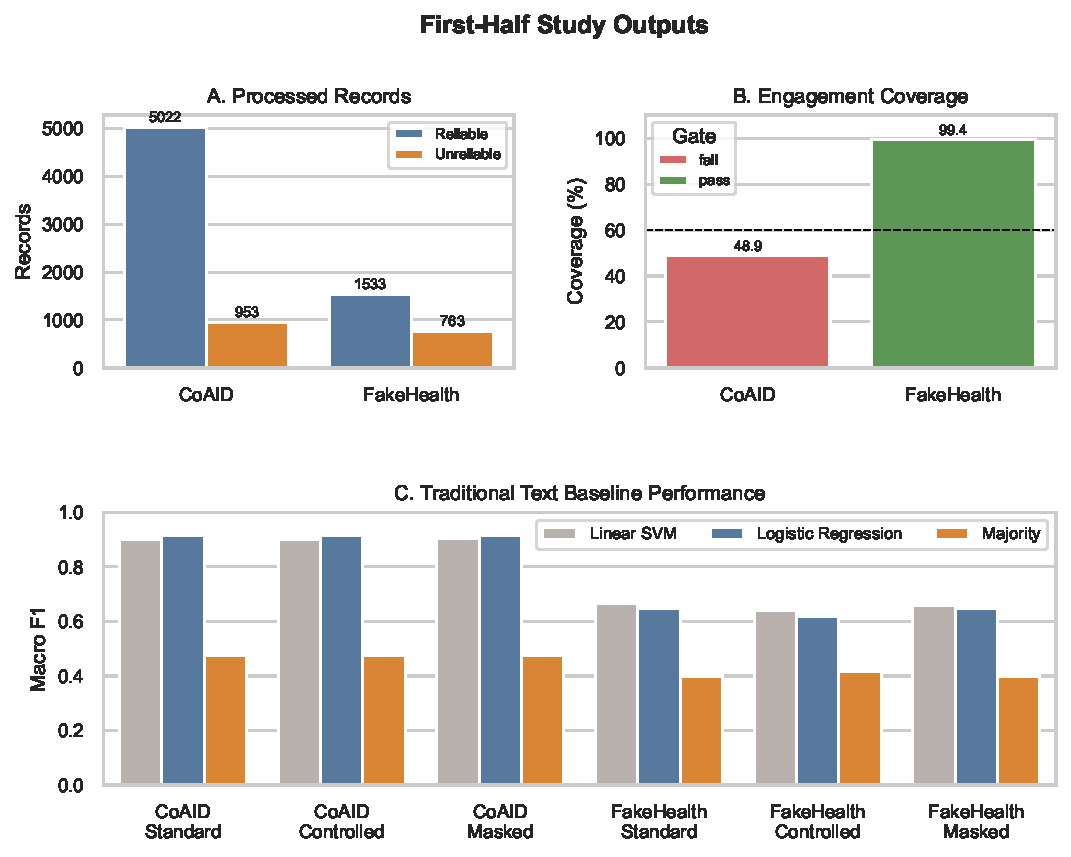
\includegraphics[width=0.72\textwidth]{figures/progress_summary_panels.pdf}
    \caption{First-half study outputs: processed records, engagement feasibility, and traditional text baseline performance.}
    \label{fig:progress-summary}
\end{figure}

\section*{Progress to Date}

The first-half implementation is complete through the traditional baseline stage and has produced local outputs for inventory, provenance, profiling, splitting, and model evaluation. The processed dataset contains 8,271 included records: 5,975 from CoAID and 2,296 from FakeHealth. As shown in Figure~\ref{fig:progress-summary}, both datasets are class-imbalanced but retain enough reliable and unreliable records for within-dataset text modeling.

The engagement feasibility analysis produced a useful early decision. CoAID failed the predictive engagement gate because usable engagement metadata covered only 48.9\% of included records and the unreliable class had only 166 engagement-complete records. FakeHealth passed the gate with 99.4\% engagement coverage, 1,526 reliable engagement-complete records, and 756 unreliable engagement-complete records. This does not yet answer whether engagement improves prediction, but it prevents the project from forcing an underpowered or biased engagement experiment on CoAID.

The split audit also produced an important methodological result. FakeHealth passed source-disjoint splitting. CoAID did not: the first source-disjoint attempt violated duplicate-family separation, so the pipeline fell back to duplicate-group stratified evaluation for CoAID. This is exactly the type of artifact-control decision the study was designed to make visible. The final split manifests guarantee that no duplicate group crosses train, validation, and test partitions.

Traditional text baselines have been run for CoAID and FakeHealth across standard, controlled, and masked-text conditions. CoAID results are strong: Logistic Regression reaches approximately 0.914 macro F1 under standard, controlled, and masked conditions, while Linear SVM reaches approximately 0.902. FakeHealth is more difficult: the best standard result is Linear SVM at approximately 0.666 macro F1, and controlled FakeHealth performance is lower. These early results support the hypothesis that within-dataset performance is dataset-dependent.

At this stage, the first research question is partially answered. Traditional text baselines are complete, but transformer comparison is not complete because the local environment lacks \texttt{torch}, \texttt{transformers}, \texttt{datasets}, and \texttt{evaluate}. The repository now contains package code, configuration files, phase scripts, tests, and documentation; raw datasets, processed tables, model outputs, and predictions remain local and ignored by Git. The next technical step is to install transformer dependencies and rerun Phase 6. The next scientific step is to compare DistilBERT against the frozen traditional baselines before moving to the second half of the study.

\newpage
\section*{References}

\aparef{Athira, A. B., Madhu Kumar, S. D., \& Chacko, A. M. (2023). A systematic survey on explainable AI applied to fake news detection. \textit{Engineering Applications of Artificial Intelligence, 122}, 106087. \url{https://doi.org/10.1016/j.engappai.2023.106087}}

\aparef{Baris-Schlicht, I., Fernandez, E., Chulvi, B., \& Rosso, P. (2023). Automatic detection of health misinformation: A systematic review. \textit{Journal of Ambient Intelligence and Humanized Computing, 15}, 2009--2021. \url{https://doi.org/10.1007/s12652-023-04619-4}}

\aparef{Chen, E., Jiang, J., Chang, H.-C. H., Muric, G., \& Ferrara, E. (2022). Charting the information and misinformation landscape to characterize misinfodemics on social media: COVID-19 infodemiology study at a planetary scale. \textit{JMIR Infodemiology, 2}(1), e32378. \url{https://doi.org/10.2196/32378}}

\aparef{Cui, L., \& Lee, D. (2020). \textit{CoAID: COVID-19 healthcare misinformation dataset}. arXiv. \url{https://arxiv.org/abs/2006.00885}}

\aparef{Dai, E., Sun, Y., \& Wang, S. (2020). Ginger cannot cure cancer: Battling fake health news with a comprehensive data repository. \textit{Proceedings of the International AAAI Conference on Web and Social Media, 14}(1), 853--862. \url{https://doi.org/10.1609/icwsm.v14i1.7350}}

\aparef{Di Sotto, S., \& Viviani, M. (2022). Health misinformation detection in the social web: An overview and a data science approach. \textit{International Journal of Environmental Research and Public Health, 19}(4), 2173. \url{https://doi.org/10.3390/ijerph19042173}}

\aparef{Langguth, J., Schroeder, D. T., Filkukova, P., Brenner, S., Phillips, J., \& Pogorelov, K. (2023). COCO: An annotated Twitter dataset of COVID-19 conspiracy theories. \textit{Journal of Computational Social Science}. \url{https://doi.org/10.1007/s42001-023-00200-3}}

\aparef{Suarez-Lledo, V., \& Alvarez-Galvez, J. (2021). Prevalence of health misinformation on social media: Systematic review. \textit{Journal of Medical Internet Research, 23}(1), e17187. \url{https://doi.org/10.2196/17187}}

\aparef{Vosoughi, S., Roy, D., \& Aral, S. (2018). The spread of true and false news online. \textit{Science, 359}(6380), 1146--1151. \url{https://doi.org/10.1126/science.aap9559}}

\aparef{Wang, Y., McKee, M., Torbica, A., \& Stuckler, D. (2019). Systematic literature review on the spread of health-related misinformation on social media. \textit{Social Science \& Medicine, 240}, 112552. \url{https://doi.org/10.1016/j.socscimed.2019.112552}}

\end{document}
